\chaptername{Vectors}
\section{Concepts of Vectors}

In this chapter, we introduce central object of the course, vectors, as well as the mathematical mental actions we will engage in to construct and analyze vectors.  The pedagogical approach of this chapter is centered around quantitative reasoning.  This pedagogical perspective is valuable for everyone, but especially relevant for STEM majors, who largely populate courses such as these.

\textbf{Lesson \ref{lesson:vectors_as_lists_of_quantities}.}  Quantities are everywhere, but we need to prepare our minds to see them.  Once we see quantities, we may begin to see lists of quantities.  The concept of vector emerges from this.

\lessonobjectives{\ref{lesson:vectors_as_lists_of_quantities}}{
\begin{checklist}
\item I understand the notions of quantity, of lists of quantities, and understand that these lists of quantities are everywhere.  
\item I can identify relevant lists of quantities from an object or situation.
\item I understand that measurements of quantities are real numbers.
\item I understand there are numerous productive metaphors for vectors and can use metaphors to interpret and give meaning to vectors.
\item Given a vector, I can correctly interpret it and communicate my thoughts in context (e.g. cereal, travel instructions, and forecasts).  
\end{checklist}
}

\textbf{Lesson \ref{lesson:symbolizing_vectors}.}  Now that we have internalized the mathematical concept of vector, we explore productive ways to symbolize vectors.  The act of symbolizing concepts in our minds is a central mathematical actions.  We go back and forth between concepts in our minds and symbols on the page.  

\lessonobjectives{\ref{lesson:symbolizing_vectors}}{
\begin{checklist}
\item Given a situation, I can symbolize relevant vectors and relationships between.
\item Given a symbolic expression involving vectors, I can interpret that expression in the context of a situation.
\item I can clearly communicate my reasoning about vectors using their names.
\end{checklist}
}

\textbf{Lesson \ref{lesson:visualizing_vectors}.}  Similar to the previous lesson, now that we have internalized the mathematical concept of vector, we explore productive ways to visualize vectors.  The act of visualizing concepts in our minds is a central mathematical actions.  There are many types of productive visualizations we will construct, including geometric and bar graph.


\lessonobjectives{\ref{lesson:visualizing_vectors}}{
\begin{checklist}
\item I understand that there are numerous visualizations for vectors, and can choose appropriate ones for a given context.
\item I can visualize a vector with list-length 2 or 3 as a point or arrow in Cartesian 2-space or 3-space.
\item I can visualize a list-length $n$ vector as a bar graph in Cartesian 2-space.
\end{checklist}
}





\newpage

%------------------------------------------------------------------------------------------------------------------
%------------------------------------------------------------------------------------------------------------------
%-------------------                       LESSON BREAK                             ----------------------------
%------------------------------------------------------------------------------------------------------------------
%------------------------------------------------------------------------------------------------------------------


\lesson{Vectors as Lists of Quantities}
\label{lesson:vectors_as_lists_of_quantities}

Welcome students!  
Before we can begin learning linear algebra, we need to establish the ontology of this book.
In this book, I take the perspective that \textbf{objects} and \textbf{situations} exist external to us everywhere.    
These objects and situations possess many types of \textbf{attributes}.   
An attribute, together with an agreed upon unit of measurement, is a \textbf{quantity}.

\spg{ %\bsp
\begin{ex}[Object-Attribute-Quantity (OAQ) Analysis of a Glass of Water]
\label{ex:oaq_water}
With my lunch, I am drinking a glass of water.  
This glass of water exists, external to me, sitting beside me on my table.  
The water has many attributes: size, mass, temperature, color, and many more.
For the moment, I will focus on its size.  
%Size is a perfectly understandable attribute, but it is not precise.  
We could agree on many ways to measure size, for example by measuring its volume in liters, cups, ounces, or cubic inches.
Let's pick ounces.
The volume of the water in my glass, measured in ounces, is a quantity.
%\begin{description}
%\item[Object/Situation:]  Glass of water
%\item[Attribute:]  Size
%\item[Quantity:]  Volume in units of ounces
%\end{description}
\vspace{-1pc}
\begin{center}
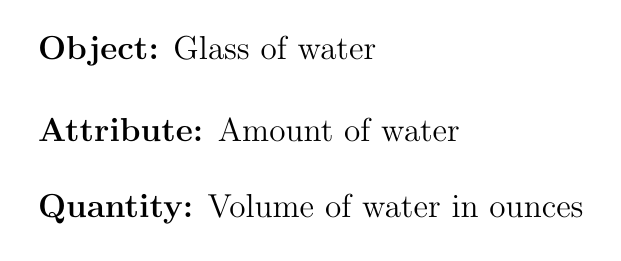
\begin{tikzpicture}
      \draw (3,3) node[anchor=west] {\large \textbf{Object:}  Glass of water};
      \draw (3,2) node[anchor=west] {\large \textbf{Attribute:}  Amount of water};
      \draw (3,1) node[anchor=west] {\large \textbf{Quantity:}  Volume of water in ounces};
\filltank{0,0}{70}
%
%\filltank[-30]{4,0}{50}
\end{tikzpicture}
\end{center}
\end{ex}
} %\esp



\spg{
\begin{activity}[OAQ Analysis]
\label{activity:oaq_analysis}
With a partner, take a few minutes to look around and identify some objects, some attributes they possess, and  agree upon a way to measure them.  After a few minutes, share some of your findings with the class.
\end{activity}
}


If I want to measure the mass of my sandwich, then I put it on a scale, select units (e.g. grams, pounds, etc), and then read off the number.
If I want to measure the distance I traveled in my car, then I look at my odometer, select units (miles or kilometers), and then read off the number.
If I want to measure the temperature at my home, then I look at my thermometer, select my units (Fahrenheit or Celsius), and then read off the number.

When we measure a quantity, we obtain a \textbf{real number}.  
For example, positive integers (e.g. 1, 2, 3, \ldots), ratios of integers (e.g. $\frac{1}{2},\frac{2}{3}$), square roots of positive integers (e.g. $\sqrt{2}$), and transcendental numbers like $\pi$ and $e$ are all real numbers.

You do not need to know the value of a real number to reason about it.  
In Example \ref{ex:oaq_water}, the volume of the water in my glass, measured in ounces is a number.  
We can reason about that volume of water without ever knowing its value.
Sometimes I will \textbf{name} a real number with an italicized lower case letter.  
For example, I might name the volume of water in my glass, measured in ounces, with the letter $v$, for volume.
I denote the collection of all real numbers as $\R$ and use the symbols $a\in \R$ to \textit{mean} $a$ is a real number.


%\newpage

\begin{vignette}[Quantities in my kitchen]
\label{vig1}
I walk into my kitchen to see what food I have to eat.
As I look through my food, I suddenly realize that they are quite literally \textit{covered} in lists of quantities!
Pretty much every packaged food item has a box called ``Nutrition Facts.''  
This box lists the masses of nutrients (either measured in grams g, milligrams mg, or micrograms mcg) contained within one serving size of the given food item.
The box always lists the masses of the three most essential nutrients called \textit{macronutrients}:  total fat, total carbohydrates, and protein.  
Sometimes masses of other nutrients such as vitamin B, vitamin C, vitamin D, calcium, iron, and potassium are also listed.

For example, the ``Nutrition Facts'' on the side of my box of Sugar-Os cereal is depicted on the right of Figure \ref{figure:kitchen}.

\spg{
\begin{figure}[H]
\centering
\begin{tabular}{p{0.58\textwidth} p{0.38\textwidth}}
%\begin{minipage}[t]{0.6\textwidth}
\vspace{0pc}\includegraphics[width=0.58\textwidth]{images/dalle/kitchen_dalle.png}&
%\end{minipage}
%\begin{minipage}[t]{0.35\textwidth}
%\centering
%\vspace{0pt}
%\textsc{\Large Sugar-Os}
\vspace{0pc}\resizebox{0.38\textwidth}{!}{\sugaros}
%\end{minipage}
\end{tabular}
\caption{Observing lists of quantities in my kitchen.}
\label{figure:kitchen}
\end{figure} 

I wonder, \textit{where else in my kitchen do I see lists of quantities}?
}
\end{vignette}


\newpage
\begin{vignette}[Quantities as I travel]
\label{vig2}
I am always driving where I need to go.  
Today alone I will drive to campus, to lunch, to the grocery store, and then home.  
Even if I know directions, I often use my GPS in case there is something like traffic or a road closure.  
As I put in my destinations today, I realize that I am staring at list of quantities!  
In a given trip, each step of the travel instructions is the distance I drive, either in miles or feet, on a given road, until I turn onto the next street.  

For example, in Figure \ref{figure:gps}, are depicted the travel instructions to get from my home to the math department.

\spg{
\begin{figure}[H]
\tikzmath{
	\XMIN = -15;
	\XMAX = 15;
	\YMIN = -7;
	\YMAX = 23;
}
\centering
\begin{tabular}{p{0.6\textwidth} p{0.38\textwidth}}
\vspace{0pc}
\begin{tikzpicture}[scale=0.33,line cap=round,line join=round,>=triangle 45,x=1cm,y=1cm,background rectangle/.style={fill=olive!15}, show background rectangle]
\clip(\XMIN,\YMIN) rectangle (\XMAX,\YMAX);
%Draw standard grid and axes
%\draw[color=geogebra_grey_light, xstep=1cm,ystep=1cm](\XMIN,\YMIN) grid (\XMAX,\YMAX);
%\draw[->,color=black] (\XMIN,0) -- (\XMAX,0);
%\draw[->,color=black] (0,\YMIN) -- (0,\YMAX);
%%Loop to draw standard coordinate labels 
%\foreach \x in {-25, -20, ..., -5,5,10,...,30}
%  \draw[shift={(\x,0)},color=black] (0pt,2pt) -- (0pt,-2pt) node[below] {\footnotesize $\x$00 ft};
%\foreach \y in {5,10,...,25}
%  \draw[shift={(0,\y)},color=black] (2pt,0pt) -- (-2pt,0pt) node[left] {\footnotesize $\y$00 ft};
%\draw[color=black] (0pt,-10pt) node[right] {\footnotesize $0$};
%Loop to draw B-coordinate grid:
\foreach \m in {-5,...,8}
  \draw [line width=2pt,color=geogebra_grey_light,domain=\XMIN:\XMAX] plot(\x,{(4/3)*(\x+4*\m)+3*\m});
\foreach \m in {-5,...,8}
  \draw [line width=2pt,color=geogebra_grey_light,domain=\XMIN:\XMAX] plot(\x,{((-3/4)*(\x-3*\m)+4*\m});
\begin{scriptsize}
%\draw [fill=g_orange] (0,0) ++(-4.5pt,0 pt) -- ++(4.5pt,4.5pt)--++(4.5pt,-4.5pt)--++(-4.5pt,-4.5pt)--++(-4.5pt,4.5pt);
\draw [fill=g_orange] (0,0) circle (15pt);
\draw[color=g_orange] (0,-2) node {\LARGE Home};
\draw[color=black] (5.5,6) node {\rotatebox{53}{\large Euclid Rd.}};
\draw[color=black] (11,11.5) node {\rotatebox{-37}{\large University Ave.}};
%\draw [color=g_purple] (23,14)-- ++(-4.5pt,0 pt) -- ++(9pt,0 pt) ++(-4.5pt,-4.5pt) -- ++(0 pt,9pt);
\draw [fill=g_purple] (23,14) circle (15pt);
\draw[color=g_purple] (27,15) node {\LARGE Bank};
%\draw [color=g_green] (5,15) ++(-4.5pt,0 pt) -- ++(4.5pt,4.5pt)--++(4.5pt,-4.5pt)--++(-4.5pt,-4.5pt)--++(-4.5pt,4.5pt);
\draw [fill=g_green] (5,15) circle (15pt);
\draw[line width=3pt, color=g_red] (0,0) -- (9,12);
\draw[->,line width=3pt, color=g_red] (9,12) -- (5,15);
\draw[color=g_green] (5,17) node {\LARGE Math Department};
\end{scriptsize}
\pic[scale=.6,fill=black,text=black] at (-8,8) {compass};
\end{tikzpicture}&
\vspace{0pc}
\textsc{\hspace{1pc} Travel Instructions}

\begin{enumerate}
\item 1500 ft on Euclid Rd. 
\vspace{2pc} 

Then take a left. 
\vspace{2pc} 
\item 500 ft on University Ave. 
\vspace{2pc}  

Then you have reached your destination.
\end{enumerate} 
\end{tabular}
\caption{Observing lists of quantities as I drive.}
\label{figure:gps}
\end{figure} 

I wonder, \textit{where else as I travel do I see lists of quantities}?
}
\end{vignette}



\newpage
\begin{vignette}[Quantities outside]
\label{vig3}
I want to plan out my day tomorrow and I look at my phone to get the forecast for the day.  
It is then that I realize that the forecast is a list of quantities!
At first I see the following table.

\vspace{-0.5pc}

\begin{center}
\begin{NiceTabular}{|l|*{8}{c|}}
\toprule
Hour        & 12am & 3am & 6am & 9am & 12pm & 3pm & 6pm & 9pm \\
\midrule
\RowStyle[nb-rows=1,color=blue]{}
\textbf{Today}& 42$^\circ$   & 39$^\circ$  & 38$^\circ$  & 48$^\circ$  & 56$^\circ$   & 59$^\circ$  & 53$^\circ$  & 46$^\circ$ \\
\bottomrule
\end{NiceTabular}
\end{center}
\vspace{-0.5pc}


%\vspace{-2pc}
I scroll down a little further and see the following visual representation.
\vspace{-0.5pc}

\tikzmath{
	\XMIN = -1;
	\XMAX = 24;
	\YMIN = 0;
	\YMAX = 70;
}
\newcommand{\mymacrotemp}{0/42, 3/39, 6/38, 9/48, 12/56, 15/59, 18/53, 21/46}
\begin{center}
\begin{tikzpicture}[scale=0.60,line cap=round,line join=round,>=triangle 45,x=0.85cm,y=0.22cm]
%Draw standard grid and axes
\draw[color=geogebra_grey_light, xstep=1cm,ystep=0.1cm](\XMIN,\YMIN) grid (\XMAX,\YMAX);
\draw[color=black, line width=2pt] (\XMIN,0) -- (\XMAX,0);
\draw[color=black, line width=2pt] (-1,\YMIN) -- (-1,\YMAX);
%Loop to draw standard coordinate labels 
\foreach \x in {0, 3,..., 21}
  \draw[shift={(\x,0)},color=black] (0pt,2pt) -- (0pt,-2pt) node[below] {\footnotesize $\x$};
\foreach \y in {10, 20, ..., 60}
  \draw[shift={(-1,\y)},color=black] (2pt,0pt) -- (-2pt,0pt) node[left] {\footnotesize $\y^{\circ}$ F};
%Loop to draw signal:
\foreach \x/\y in \mymacrotemp
  \draw [line width=2pt,color=blue] (\x,0)--(\x,\y) node[above] {$\y^{\circ}$ F};
%\begin{scriptsize}
\draw[color=black] (12,-5.5) node[below] {\large Hours After Midnight};
\draw[color=black] (-5,30) node[below, rotate=90] {\large Temperature};
%\end{scriptsize}
\end{tikzpicture}
\end{center}

\vspace{-1.5pc}

I really like being able to see both the table and the visual.
The table is nice and concise, but the visual gives me an excellent sense of how the temperature varies.  

I wonder, \textit{what other lists of quantities are useful in describing the weather}?

\end{vignette}





%\newpage
%
%
%\begin{discussion}
%Read the vignettes and discuss in groups the following questions.
%\vspace{-1pc}
%\begin{enumerate}
%\item  What do these vignettes have in common?
%\item ADDRESS EACH WONDERING?
%\end{enumerate}
%\end{discussion}
%

\newpage
Observe that in each vignette, we encountered many quantities, naturally grouped together, all at once.

\spg{ %\bsp
\begin{Def}[Lists and List-Length]
\label{def:lists}
A \textbf{list of quantities} is an ordered collection of quantities.  
The number of entries in the list is its \textbf{list-length}.
\end{Def}
} %\esp

Lists of quantities are united, tied together, by a single object or situation.  


\spg{ %\bsp
\begin{ex}[List of Quantity Analysis of \textbf{Vignette \ref{vig1}}]  
\label{ex:vignettes1}
%
An \textbf{object} here is one serving size of cereal. \\

An \textbf{attribute} of one serving size of cereal is nutrition.  
I can measure nutrition in many ways, for example: grams of fat, grams of carbs, grams of protein, etc.
The \textit{list of macronutrients}, below left, has list-length 3.\\

A different \textbf{attribute} is my daily consumption.
I can quantify consumption in many ways, for example: the number of serving sizes I consume each day of the week.
The list of servings consumed, below right, is a list of list-length 7.


\begin{center}
\begin{minipage}[t]{0.43\textwidth}
\small
\begin{todos}[frametitle={\textsc{Macronutrient List}}]
\begin{enumerate}[leftmargin=0.5pc]
\item Grams of fat in one serving size, 
\item Grams of carbs in one serving size, 
\item Grams of protein in one serving size.
\end{enumerate}
\end{todos}
\normalsize
\end{minipage}
%\begin{minipage}[t]{0.01\textwidth}
%${}$
%\end{minipage}
\begin{minipage}[t]{0.56\textwidth}
\small
\begin{todos}[frametitle={\textsc{Daily Consumption List}}]
\begin{enumerate}[leftmargin=0.5pc]
\item Number of serving sizes consumed on Sunday, 
\item Number of serving sizes consumed on Monday,
\item Number of serving sizes consumed on Tuesday,
\item Number of serving sizes consumed on Wednesday,
\item Number of serving sizes consumed on Thursday,
\item Number of serving sizes consumed on Friday,
\item Number of serving sizes consumed on Saturday.
\end{enumerate} 
\end{todos}
\normalsize
\end{minipage} 
\end{center}
 \vspace{1pc}
%
%\#Monday, \ldots, \#Saturday] is a list of list-length 7.\\
\end{ex}
} %\esp


\spg{ %\bsp
\begin{ex}[Revisiting our vignettes with our new lens of lists of quantities.]
\label{ex:vignettes2}

\textbf{Vignette \ref{vig2}.}
The situation is the collection of places near my home.
An attribute of this situation is distances between places.
I can quantify distances in many ways, for example: feet east/west, feet north/south, number of blocks, etc.
The list of cardinal direction distances, [feet east, feet north], is a list of quantities of list-length 2.\\

A different attribute is population density.
I can quantify population density in many ways, for example, number of people who live in a given block.
Supposing I number each block, and my neighborhood has 40 blocks, then the list of populations per block has list-length 40.
\end{ex}
} %\esp



\spg{ %\bsp
\begin{ex}[List of Quantity Analysis of \textbf{Vignette \ref{vig3}}]  
\label{ex:vignettes3}
An \textbf{object} is the air outside my home.\\

An \textbf{attribute} of air is temperature.  
I can quantify temperature in many ways, for example measure the temperature in degrees Fahrenheit in 3 hour intervals throughout the day.
The \textit{list of temperatures}, below left, has list-length 8.\\

A different \textbf{attribute} is humidity.
I can quantify humidity in many ways, for example measure the relative humidity (in percents) in 4 hour intervals throughout the day.
The \textit{list of humidities}, below right, has list-length 6.

\begin{center}
\begin{minipage}[t]{0.35\textwidth}
\small
\begin{todos}[frametitle={\textsc{Temperature List}}]
\begin{enumerate}[leftmargin=0.5pc]
\item Degrees Fahrenheit at 12am,
\item Degrees Fahrenheit at 3am,
\item Degrees Fahrenheit at 6am,
\item Degrees Fahrenheit at 9am,
\item Degrees Fahrenheit at 12pm,
\item Degrees Fahrenheit at 3pm,
\item Degrees Fahrenheit at 6pm,
\item Degrees Fahrenheit at 9pm.
\end{enumerate}
\end{todos}
\normalsize
\end{minipage}
\begin{minipage}[t]{0.05\textwidth}
${}$
\end{minipage}
\begin{minipage}[t]{0.35\textwidth}
\small
\begin{todos}[frametitle={\textsc{Relative Humidity List}}]
\begin{enumerate}[leftmargin=0.5pc]
\item Percent humidity at 12am,
\item Percent humidity at 4am,
\item Percent humidity at 8am,
\item Percent humidity at 12pm,
\item Percent humidity at 4pm,
\item Percent humidity at 8pm.
\end{enumerate}
\end{todos}
\normalsize
\end{minipage} 
\end{center}
 \vspace{1pc}

\end{ex}
} %\esp
%
%
%Let us look back at our vignettes.
%
%In Vignette \ref{vig1}, my box of cereal is an object. 
%An attribute my box has is its nutrition.  
%I can quantify nutrition in many ways, for example: grams of fat, grams of carbs, grams of protein, etc.
%
%In Vignette \ref{vig2}, 
%In Vignette \ref{vig2}, an object is the air outside my home.
%An attribute this object has is temperature.
%I can quantify temperature in many ways, for example: degrees Fahrenheit at 12am, degrees Fahrenheit at 3am, etc.

\newpage
\spg{ %\bsp
\begin{action}[Identifying Structures]
Identifying structures is the act of analyzing an object or situation and picking out specific features.  
\end{action}

Right now, we are interested in analyzing objects and situations and identifying lists of quantities.  
}

\bsp
\begin{activity}[Identifying Lists of Quantities]
\label{activity:identifying_lists_of_quantities}
Consider each of the following situations.
With a partner, write down several lists of quantities that might naturally come up when analyzing the situation.
Be sure to clearly specify each quantity (include object, attribute, and agreed way to measure).  
Note that these are intentionally vague and open-ended prompts.
\begin{enumerate}[label=(\alph*)]
\item \textit{The most recent time you went grocery shopping.}
\item \textit{Your phone.}
\item \textit{Your social media account.}
\item \textit{The houses on your block.}  
\item \textit{A recording of a song by your favorite band.}
\item \textit{The voting precincts in your region.}
\item \textit{A single website that is comprised of 17 distinct pages.}
\item \textit{Your favorite sports team.}
%\item 
%\textit{There is a major city called Mathopolis and an adjacent suburb called Vector Valley.}  
%\item 
%\textit{In a linear algebra class, starting at 2pm, with 30 students present, the instructor hands out an exam.}
%\item 
%\textit{A 10 person jazz band starts playing their opening piece of a performance.}
\end{enumerate}
\end{activity}  
\esp  

Lists of quantities are so important, we encode this idea within a single term: vector.

\begin{Def}[Vector]
\label{def:vector}
A \textbf{vector} is an (ordered) list of quantities.  The \textbf{list-length} of a vector is the length (i.e. number of entries) in its associated list.
\end{Def}

\vspace{-1pc}
Throughout our day, we are constantly coming across vectors: nutrition facts in cereal, prices of our groceries, populations in cities, temperatures outside, internet search rankings, and even the color data for the pixels on our electronic displays.  In fact, a single image on a 4K LCD display is encoded within a list of $3\times 3840 \times 2160 = 24,883,200$ many numbers!
%, i.e., an image is a vector in 
%
%$\R^{24,883,200}$.)  

\spg{ %\bsp
\begin{psa}[Meaningful vectors can have large list-length!]
\label{psa:large_list_length}
%The list-length of important vectors can be quite large.
People often think of vectors as only being geometric coordinates and limit their thinking to list-lengths of 1, 2, or 3.  
While these are important examples of vectors, they can also constrain our thinking.
I hope you see already that vectors of potentially large list-length are \textit{natural} and \textit{everywhere}.
\end{psa}
} %\esp


\newpage
\bsp
\begin{activity}[Constructing Feature Vectors (Machine Learning)]
\label{activity:feature_vector}
In Figure \ref{fig:miyagi} is a photo of my very sweet cat.   
In a quick glance, I can recognize him.

\begin{figure}[H]
\centering

\includegraphics[width=0.45\textwidth]{images/miyagi.jpg}

\includegraphics[width=0.45\textwidth]{images/miyagi-snout.png}
\caption{(Left) A photo of my cat.  (Right) Image depicting Snout-Eye ratio.}
\label{fig:miyagi}
\end{figure}

\vspace{-0.5pc}

I bet many of you have cats and dogs too.  
Pull up some pictures of them for this activity.
When you look at them, you probably do not have any difficulty identifying which photos are of cats and which photos are of dogs.
\textit{How do you think a computer might be able distinguish between photos of cats and photos of dogs?}

\vspace{0.4pc}

Computers cannot analyze images like we can - we need to tell them what to look for.
%This is exactly what happens in the area of Machine Learning.
We need to identify a list of useful quantities from which the computer can learn to make the distinction between cats and dogs.
% classification.
In the area of machine learning, this emergent vector is sometimes called a \textbf{feature vector}.

\vspace{0.4pc}


Let me give you an example of one quantity we may wish to include in our feature vector.
Usually (but not always) dogs have longer snouts than cats, so snout length is a promising attribute to include in our feature vector.
Unfortunately we cannot measure the \textit{absolute} length of the snout from the photo, since we do not know the scale of the photo.  
Instead, we could measure the \textit{relative} length of the snout compared to the distance between the eyes. 
For each photo, computers can compute and record this \textit{snout-to-eye} ratio.

\vspace{0.4pc}

While this is a promising quantity, it is probably not enough for the computer the learn the difference between cats and dogs.  
(Why do you think this is the case?)  
In groups, come up with other promising quantities which you can read from a picture, and for which will be useful in trying to tell the difference between cats and dogs.

\vspace{0.4pc}

When you are done, share with the class your feature vector.  
What quantities comprise your feature vector?  
What is its list-length?  
Do you think that you have given the computer enough quantities that it should be able to distinguish pictures of cats from pictures of dogs by looking at their feature vectors?

\vspace{0.4pc}

Feature vectors form the starting point for machine learning. 
\end{activity}
\esp
\vspace{-0.5pc}




%------------------------------------------------------------------------------------------------------------------
%------------------------------------------------------------------------------------------------------------------
%-------------------                       LESSON BREAK                             ----------------------------
%------------------------------------------------------------------------------------------------------------------
%------------------------------------------------------------------------------------------------------------------
\newpage
\lesson{Symbolizing Vectors}
\label{lesson:symbolizing_vectors}

\spg{
Let's begin this lesson by returning to cereal.  
In Figure \ref{figure:cereals_symbolize} are the nutrition facts for Sugar-Os.
\vspace{-1pc}

\begin{figure}[H]
\centering
\begin{tabular}{p{0.67\textwidth} p{0.3\textwidth}}
%\begin{minipage}[t]{0.6\textwidth}
\vspace{0pc}\includegraphics[width=0.67\textwidth]{images/pd/bowl-of-cereal-with-strawberries.jpeg}&
%\end{minipage}
%\begin{minipage}[t]{0.35\textwidth}
%\centering
%\vspace{0pt}
%\textsc{\Large Sugar-Os}
\vspace{0pc}\resizebox{0.3\textwidth}{!}{\sugaros}
%\end{minipage}
\end{tabular}
\caption{Sugar-Os Cereal}
\label{figure:cereals_symbolize}
\end{figure}

\vspace{-1pc}

\textit{How can I efficiently communicate lists of quantities such as the nutrition facts for one serving size of cereal?}
It is desirable to do so without writing having to write out long lists like those in Example \ref{ex:vignettes1}?  
A core mathematical act is to create and use symbols to organize our thoughts and communicate our reasoning.  
}

\newpage
\spg{ %\bsp
\begin{action}[Symbolizing]
\label{mental_action:symbolizing}
Symbolizing is the act of associating a concept in our minds with a symbol on the page.  
\textit{Note that we first need a concept in our minds!}
For example, the concept of five can be symbolized 5, or V (Roman numerals), or 101 (binary).    
Depending on the context, we choose the symbolization that is most appropriate, that enables us to communicate, to reason, or to solve a specific problem.
\end{action}
} %\esp

Let's explore some productive ways to symbolize vectors by focusing first on the vector of nutrition facts for a single serving size of Sugar-Os.

To begin, we may concretely symbolize the nutrient facts with a vertical \textbf{column} of all the numbers associated with the quantities.
%In so doing, we can concretely write down the list of numbers. %and then compute the nutrients in the mixture.
%\spg{ %\bsp
%\begin{notation}[Writing vector entries]
%For reasons that will become clearer later, if we want to write down the entries in our list, then we will write our lists \textit{vertically}.
%So to symbolize one serving size of Sugar-Os, I will write a \textbf{column} for the vector
%
%$$\begin{bmatrix}1.6\\199\\31\\2.1\\1.3\\132\\6\\92\end{bmatrix}.$$
%
In column form, I typically do not write down the units, but I remember they are still there.  
Each number in the column is an \textbf{entry}
This way of symbolizing this vector is useful because I can efficiently see all the quantities and I can use this for numerical computations.  
%We will usually use the same letter for the vector name as for the vector entries, except vector entries will not be bold and will have subscripts to denote their position in the list.  
%For example, if $\vect{v}$ is a vector of list-length 4 and if we want to write the entries of $\vect{v}$, we will usually write $\vect{v}=\begin{bmatrix}v_1\\v_2\\v_3\\v_4\end{bmatrix}$.
%
%You may encounter context where people write their vector entries in different ways, for example horizontally, and maybe with parentheses or angle-brackets instead of brackets, e.g. $[v_1, v_2, v_3, v_4]$, $(v_1, v_2, v_3, v_4)$, or $\langle v_1, v_2, v_3,v_4\rangle$.
%For your work with this text, please use vertical notation when writing a vector with its entries.
%\end{notation}
%} %\esp

However, columns can be cumbersome, and in certain situations, I may not need to know the nutrient values to reason about them or to talk about them.  
For example, I can talk to you about Sugar-Os without telling you explicitly the nutrient facts.
Just as we have a name for cereal, it is useful to also have a \textbf{name} for a vector.  
I will always name vectors with a single, lowercase bold letter.  In this case, I will choose $\textbf{s}$ to help me remember this vector comes from \textbf{S}ugar-Os.
The symbolizing just described is summarized in Figure \ref{figure:symbolizing}.

\spg{ %\bsp
\begin{figure}[H]
\centering
\begin{tikzpicture}[scale=1, line cap=round,line join=round,>=triangle 45,x=1cm,y=1cm,decoration={
    markings,
    mark=at position 1 with {\arrow{>}}}]
	 \draw [ultra thick, black] (2.5,0.5) edge[bend left=-20,looseness=0.8,postaction={decorate}]  node[above, sloped] {\Large Symbolize} node[below, sloped] {Column} (7.4,2);
	 \draw [ultra thick, black] (2.5,-0.5) edge[bend left=20,looseness=0.8,postaction={decorate}]  node[below, sloped] {\Large Symbolize} node[above, sloped] {Name} (7.4,-2);
      \draw (0,0) node {\resizebox{0.3\textwidth}{!}{\sugaros}};
      \draw (8,2) node {$\begin{bmatrix}1.6\\199\\31\\2.1\\1.3\\132\\6\\92\end{bmatrix}$};
      \draw (8,-2) node {\Large$\vect{s}$};
      \draw (0,4.2) node {\textsc{\Large  Sugar-Os}};
      \end{tikzpicture}
\caption{Symbolizing vectors in two ways:  \textbf{column} and \textbf{name}.}
\label{figure:symbolizing}
\end{figure}
} %\esp


\spg{ %\bsp
\begin{notation}[Vectors]
\label{notation:vectors}
\begin{sectionlist}
\bitem{Writing names.} 
I will always name vectors with a single, lowercase bold letter.
When typing, please do the same.
When writing by hand, bold font is impractical, so please always use the notation of a right-pointing arrow over the symbol: $\vec{v}$.

\bitem{Relating the symbols for name and entries.}
I will usually use the same letter for the vector name as for the vector entries, except entries will not be bold and will have subscripts to denote their position in the list.  
For example, if I want to write the entries of a list-length 3 vector named $\vect{v}$, I will usually write $\vect{v}=\begin{bmatrix}v_1\\v_2\\v_3\end{bmatrix}$.  
In Figure \ref{figure:symbolizing}, I denote entries of $\vect{s}$  by $s_i$, where $i\in \{1,2,\ldots, 8\}$, and for instance, since the third entry has value 31, I would write $s_3=31$.
  
\bitem{Why a column and not a row?}  
For reasons that will become clearer later when we discuss matrix multiplication as transformation in Lesson \ref{lesson:matrix_transformation}, it is best to write entries in a vertical column instead of in a horizontal row.

\bitem{Different Books, Different Notations.} 
You may encounter contexts where people write their vector entries in different ways, for example horizontally, and maybe with parentheses or angle-brackets instead of brackets, 
e.g. $[v_1, v_2, v_3]$, $(v_1, v_2, v_3)$, or $\langle v_1, v_2, v_3\rangle$.
For your work with this text, please use vertical column notation when writing a vector with its entries.

\bitem{Consistency is important.}  
Consistency of notation brings clarity to your writing.  Please follow the above notational guidelines and always be consistent with how you write your vector names and columns.
\end{sectionlist}
\end{notation}
} %\esp
%
%\begin{notation}[Naming vectors]
%In this text, we will always name vectors with a single, lowercase bold letter.
%When typing, please do the same.
%When writing by hand, bold font is impractical, so please always use the notation of a right-pointing arrow over the symbol: $\vec{v}$.
%\end{notation}



%\spg{ %\bsp
%\begin{notation}[Writing vector entries]
%For reasons that will become clearer later, if we want to write down the entries in our list, then we will write our lists \textit{vertically}.
%We will usually use the same letter for the vector name as for the vector entries, except vector entries will not be bold and will have subscripts to denote their position in the list.  
%For example, if $\vect{v}$ is a vector of list-length 4 and if we want to write the entries of $\vect{v}$, we will usually write $\vect{v}=\begin{bmatrix}v_1\\v_2\\v_3\\v_4\end{bmatrix}$.
%
%You may encounter context where people write their vector entries in different ways, for example horizontally, and maybe with parentheses or angle-brackets instead of brackets, e.g. $[v_1, v_2, v_3, v_4]$, $(v_1, v_2, v_3, v_4)$, or $\langle v_1, v_2, v_3,v_4\rangle$.
%For your work with this text, please use vertical notation when writing a vector with its entries.
%\end{notation}
%} %\esp

When we move between a vector's name and a vector's column of entries, I will say we are \textbf{unpacking} or \textbf{repacking} the vector.  
Think of the name as a \textit{backpack}, and the entries as its \textit{contents}.


%\newpage
%
%\begin{activity}
%Think of an object or situation you encounter in your life that is actually a list of quantities.  
%(Be sure to pick one using different lists of quantities from the vignettes above.)  Clearly describe the object or situation and the associate list of quantities.  Does it make sense to add such lists?  
%If so, what would that mean in context?  
%Does it make sense to scale such a list?  
%If so, what would it mean in context?
%\end{activity}

\spg{
\begin{activity}[Discussion]
\label{activity:vectors:name_and_column}
\begin{enumerate}
\item Suppose $\vect{v}=\begin{bmatrix}1\\2\\3\end{bmatrix}$.
With a partner discuss the following.
\begin{enumerate}[label=(\alph*)]
\item When is it advantageous to work with its name $\vect{v}$?
\item When is it advantageous to work with the column of its entries $\begin{bmatrix}v_1\\v_2\\v_3\end{bmatrix}$?
\end{enumerate}
\item Suppose you have a vector with name $\vect{w}$, but you do not know its entries.  In what ways can you still work with $\vect{w}$?  In this context, what are the limitations on working with $\vect{w}$?
\end{enumerate}
\end{activity}
}

%When we move between a vector's name a vector's column of entries, I will say we are \textbf{unpacking} or \textbf{repacking} the vector.  
%You can think of the name as a \textit{backpack}, and the entries are its contents.
%

%
%\spg{ %\bsp
%\begin{ex}\label{ex:cereal}
%One of my favorite examples of vectors is cereal!  
%Look at the side of your favorite cereal box and find the \textit{Nutrition Facts}.
%This is a standardized list of numbers as mandated by the Food and Drug Administration (FDA).
%
%\begin{minipage}[t]{0.4\textwidth}
%
%    The Nutrition Facts box provides a list of masses of certain nutrients contained within a single serving size of your cereal. \\ 
%    
%    In the case to the right, the masses of nutrients contained within a serving size of this cereal is a vector of list-length 12.  Since this vector is a single serving size, I will name it $\vect{s}$.\\
%    
%    Note that implicitly I am keeping track of units and the order in which I wrote down the numbers.  For example, $s_4=160$ (mg of sodium)  and $s_9=2$ (mcg of Vitamin D).\\
%    
%\end{minipage}
%\begin{minipage}[t]{0.06\textwidth}
%    ${}$
%\end{minipage}
%\begin{minipage}[t]{0.3\textwidth}
%\vfill
%\vspace{-1.6pc}
%\resizebox{\textwidth}{!}{
%    \sffamily
%    \fbox{%
%    \begin{tabular}{@{}p{\NFwidth}@{}}
%        \NFtitle\\
%        \NFrule
%        \NFtext{8 Servings Per Container}\\
%        \NFtext{\bfseries Serving Size \hfill  2/3 cup (55\,g)}\\
%        \NFRULE
%        \NFline{\bfseries Amount Per Serving}\\
%        \NFline{\bfseries \Large Calories \hfill 230}\\
%        %\NFelement{Calories}{20}{Calories from Fat 10}\\
%        \NFRule
%        \NFline[r]{\textbf{\% Daily Value*}}\\
%        \NFrule
%        \NFelement{Total Fat}{8\,g}{10\%}\\
%        \NFsubelement{Saturated Fat}{1\,g}{5\%}\\
%        \NFsubelement{\textit{Trans} Fat}{0\,g}{0\%}\\
%        \NFrule
%        %\NFelement{Cholesterol}{0\,g}{0\%}\\
%        %\NFrule
%        \NFelement{Sodium}{160\,mg}{7\%}\\
%        \NFrule
%        \NFelement{Total Carbohydrate}{37\,g}{13\%}\\
%        \NFsubelement{Dietary Fiber}{4\,g}{14\%}\\
%        \NFsubelement{Total Sugars}{12\,g}{20\%}\\
%        \NFrule
%        \NFelement{Protein}{3\,g}{6\%}\\
%        \NFRULE
%        \NFmicroelement{Vitamin D}{2\,mcg}{10\%}\\
%        \NFmicroelement{Calcium}{260\,mg}{20\%}\\
%        \NFmicroelement{Iron}{8\,mg}{45\%}\\
%        \NFmicroelement{Potassium}{240\,mg}{6\%}\\
%        \NFrule
%        \NFtext{\tiny * The \% Daily Value (DV) tells you how much nutrient in a serving of food contributes to a daily diet.
%        2,000 calories a day is used for general nutrition advice.}
%    \end{tabular}}
%    \rmfamily
%}
% 
%%\includegraphics[width=\textwidth]{images/nutrition_facts.png} 
%\end{minipage}
%\begin{minipage}[t]{0.15\textwidth}
%    $$\Longrightarrow \ \ \vect{s}=\begin{bmatrix}8\\1\\0\\160\\37\\4\\12\\3\\2\\260\\8\\240\end{bmatrix}.$$
%\end{minipage}
%%
%%    Throughout the rest of the course, I will be referencing the language of this example.  It will be a powerful and productive \textbf{metaphor} to organize and communicate our thoughts.
%
%\end{ex}
%} %\esp
%
%
   
%  \textit{Can you think of other examples of vectors you see in your day-to-day life?}
  

%
%\begin{ex}
%Continuing Example \ref{ex:vignettes1},
%our macronutrient list lies in $\R^3$, 
%our cardinal direction distance list lies in $\R^2$,
%and our forecast list lies in $\R^8$.
%\end{ex}
  


%\fbox{
%\begin{minipage}{1\textwidth}
%By the end of this section, students should come to understand the notion of quantity, of lists of quantities, and understand that these lists of quantities are everywhere.  Students should see that under appropriate circumstances, it is meaningful to add and scale these lists.
%Students should understand the measurements of quantities are real numbers and that lists of real numbers are vectors.
%Students should see a vector as a single whole.
%\end{minipage}
%}


\newpage

%We then discuss this activity as a class.  
%This discussion includes being explicit about stating the quantities of each vector, clearly naming each vector, and identifying its list-length.


Let's return to the context of food.
Each food has its own macronutrient list.  
As you think about all the different foods you encounter each day, imagine the thousands upon thousands of macronutrient lists that there must exist.
It is useful for us to introduce symbols to denote the collection of all possible lists of a given list-length.  
We will do so using the language and notation of sets.

The language and notation of sets is foundational in mathematics.  
In the rest of this course, we will frequently use set notation to compactly represent our thoughts.
A set is a collection of objects, which we call \textbf{elements} of that set.  

Just like vectors, we can symbolize sets with either their \textbf{name} or with the \textbf{collection} of its objects, which we group together with ``curly brackets'' $\{$ and $\}$.  
For example, in the RGB color model, the three primary colors are: \textcolor{red}{red}, \textcolor{green!80!black}{green}, and \textcolor{blue}{blue}.  
I could denote this set of primary colors with the collection: \{\textcolor{red}{red}, \textcolor{green!80!black}{green}, \textcolor{blue}{blue}\} or I could name it, say with the letter $C$ (for color), in which case I would write
$$C = \{\mbox{\textcolor{red}{red}, \textcolor{green!80!black}{green}, \textcolor{blue}{blue}}\}.$$

%\begin{notation}[Set Notation]

A standard way to write a set of all elements $P$ satisfying some condition $Q$ is $\{P \ | \ Q\}$.  
The vertical bar here is understood to represent the words ``such that'' and I read this aloud as ``the set of all elements $P$ such that $Q$.''  
This set notation is a particularly important way to symbolize sets that have infinitely many elements.
\label{notation:set}
%We will use this notation frequently throughout the text.
%\end{notation}

%\vspace{-1pc}

\begin{Def}[Vector Space $\R^m$]
\label{def:vector_space}
If $m$ is a positive integer, then the set of all list-length $m$ vectors is the \textbf{vector space} $\R^m$ (read ``R  m'').  
In symbols, using set notation, I write $\R^m$ as 
$$\R^m \defeq \{ \vect{v} \ | \ \vect{v} \mbox{ is a vector with list-length } m \}.$$
Read aloud, I say ``R m is the set of all vectors v such that v is a vector of list-length m.'' The $\R$ come from $\R$eal numbers, and reminds us that the entries of the lists are real numbers.
\end{Def}

I will frequently use two other set symbols: $\in$ and $\subset$.  

The symbol ``$\in$'' means \textit{is an element of}.  
The symbol $\in$ describes a relationship between a set and individual elements of that set.  
So the expression
$\vect{v}\in\R^{17}$ means that $\vect{v}$ is an element of the set of $\R^{17}$, and hence $\vect{v}$ is a list-length 17 vector.
A slash through the symbol negates the symbol.  
So $\vect{w}\not\in\R^{34}$ would mean that $\vect{w}$ is \textit{not} a list-length 34 vector.  

The symbol ``$\subset$'' means \textit{is a subset of}.  
The symbol $\subset$ describes a relationship between a set and subsets of that set.  
So the expression
$S \subset \R^{17}$ means that $S$ is an subset of the set $\R^{17}$, and hence $S$ is collection of list-length 17 vectors.
A slash through the symbol negates the symbol.  
So $T\not\subset\R^{34}$ would mean that $T$ is \textit{not} a collection of list-length 34 vectors.  

Throughout the course, I will use both $\in$ and $\subset$ frequently and move between them.  For example,
I may write either $\vect{v}_1,\ldots, \vect{v}_8\in \R^{12}$  or  $\{\vect{v}_1,\ldots, \vect{v}_8\} \subset \R^{12}$ to say that 
$\vect{v}_1$ through $\vect{v}_8$ are list-length 12 vectors.


\newpage

\bsp
\begin{action}[Interpreting Symbols]
\label{mental_action:interpretting}
%What is \textit{symbolizing}?  
Interpreting symbolism is the act of taking a symbolic expression and understanding it in the context of a specific situation.
This is a process that happens in our minds, but we often will need to then clearly communicate our interpretation to others.

\vspace{0.5pc}

Interpreting symbols is highly dependent upon the context in which we are working.
Consider for example, the symbols $5+3$.
In the context of number of people, this can be interpreted as: \textit{the number of people when you combine a group of 5 people with a group of 3 people.}
In the context of minutes elapsed since lunch, this is interpreted as \textit{5 minutes elapsed and then 3 more minutes elapsed.}
\end{action}
\esp




\bsp
\begin{activity}[Interpretation of Vectors in Context]
\label{activity:interpretting_vectors}
Consider the vector $\vect{v}=\begin{bmatrix}3\\2\\1\end{bmatrix}$.
In each of the following contexts, explain in complete sentences a meaning of this vector.   
If there is ambiguity in the context, explain and provide potential clarification.
\begin{enumerate}[label=(\alph*)]
\item Macronutrients (in grams) for a cereal.  (For a reminder about macronutrients, see Example \ref{ex:vignettes1}.)
\item Directions (in feet) to reach a book on your bookshelf.
\item Prices (in \$) of grocery items.
\end{enumerate}
In which of these contexts could the vector $\vect{w}=\begin{bmatrix}4\\3\\2\\1\end{bmatrix}$ make sense?
\end{activity}
\esp


\bsp
\begin{activity}[Interpretation of Set Notation]
\label{activity:interpretting_set_notation}
Interpret each of the following expressions involving vector names ands set notations.  Explain their meaning.
\begin{enumerate}[label=(\alph*)]
\item $\vect{b} \in \{\vect{a}, \vect{b}, \vect{c}\}$
\item $\{\vect{x}, \vect{y}, \vect{z}\}\subset \R^{23}$
\item $\begin{bmatrix}1\\0\end{bmatrix}\in  \R^2$
\item $\begin{bmatrix}1\\0\end{bmatrix}\not\in  \R^3$
\item $X  = \{\vect{v}\in \R^{19}| v_3 = 0\}$ 
\end{enumerate}
\end{activity}
\esp


\newpage
To conclude this lesson, keep in mind that symbols are meaningless without the associated concepts in our minds.  
It was a pedagogical decision to first focus on constructing the concept of vector in Lesson \ref{lesson:vectors_as_lists_of_quantities} and then only afterwards, introduce symbolism to help us reason about and communicate our thinking about vectors.  Associated to this, you will need to both symbolize vectors (which other can then interpret) and interpret this symbolism of others (Figure \ref{figure:symbolize}).

\begin{figure}[H]
\centering
\includegraphics[width=\textwidth]{images/chp1_symbolize.png}
\caption{Symbolize and Interpret as Communication}
\label{figure:symbolize}
\end{figure}

%Furthermore, this aides with the encapsulation of a vector as a single object.
%We can unpack a vector and get list of potentially large length.
%After resolving this activity, we practice interpreting symbols within the context of a given situation.  
%This can be understood as practice moving from the symbolic world back to the embodied world \cite{tall2008}.
%I have students work in groups on a task such as that in Activity \ref{activity:interpretting_symbolism}.
%\\





%------------------------------------------------------------------------------------------------------------------
%------------------------------------------------------------------------------------------------------------------
%-------------------                       LESSON BREAK                             ----------------------------
%------------------------------------------------------------------------------------------------------------------
%------------------------------------------------------------------------------------------------------------------
  
\newpage 
\lesson{Visualizing Vectors}
\label{lesson:visualizing_vectors}

What images do you think of when you picture a serving size of cereal?  
What images do you think of when you picture a vector?    

\spg{ %\bsp
\begin{action}[Visualizing]
\label{mental_action:visualizing}
Visualizing is the act of associating a concept in our minds with images.  
For example, the concept of five can be visualized with an image of 5 objects or with the image of 5 on the number line.
Depending on the context, we choose the visualization that is most appropriate, that enables us to communicate, to reason, or to solve a specific problem.
\end{action}
} %\esp

Vectors are lists of quantities.
%They do not inherently come with any particular metaphor.
They do not inherently come with any particular geometry or visualization.
However, there are a few powerful visualizations that I will explicitly identify now to help you in your reasoning and communication.
%I group these in two two types of metaphors: \textit{action metaphors} and \textit{visualization metaphors}.

%\subsubsection{Action Metaphor 1: Vectors as Cereal}
%When using this metaphor, think of a vector $\vect{v}$ as representing a the list of nutritional content of single serving size of a box of cereal.  
%This enable us to think about such actions as adjusting serving sizes and mixing different cereals.
%See, for example, Vignette \ref{vig1} and Example \ref{ex:cereal}.
%
%\subsubsection{Action Metaphor 2: Vectors as Travel Instructions}
%When using this metaphor, think of a vector $\vect{v}$ as representing the travel instructions to reach a destination from your current location.  
%Each entries represents a distance you need to travel in a specific direction, measured in steps or feet or meters, etc.
%This enable us to think about such actions as going forwards and backwards.
%See, for example, Vignette \ref{vig2}. %and Example \ref{ex:cereal}.
%%
%%couple distinct visualizations that help support reasoning about vectors.


\subsubsection{Geometric Visualizations: Vectors as Points or Arrows}

\vspace{-1pc}
In geometric visualizations, we view the entries of a vector as \textit{spatial} coordinates.

This representation is most easily seen for the \textbf{Cartesian plane} (a.k.a. \textbf{Cartesian 2-space}).  
Here, a list of two numbers describes points on the plane, where the first number gives your horizontal position, and the second number gives your vertical position.
Given a vector $\vect{v}\in\R^2$, sometimes it is productive to think of it as a \textbf{point} in the Cartesian plane, and sometimes it is productive to think of it as the \textbf{arrow} originating at the \textit{origin} $(0,0)$ (its \textit{tail}) and going to the point (its \textit{tip}).

%\begin{figure}[h]
%\centering
%\begin{tikzpicture}[scale=1, line cap=round,line join=round,>=triangle 45,x=1cm,y=1cm,decoration={
%    markings,
%    mark=at position 1 with {\arrow{>}}}]
%	 \draw [ultra thick, black] (2.5,0.5) edge[bend left=-20,looseness=0.8,postaction={decorate}]  node[above, sloped] {\Large Symbolize} node[below, sloped] {Column} (7.4,2);
%	 \draw [ultra thick, black] (2.5,-0.5) edge[bend left=20,looseness=0.8,postaction={decorate}]  node[below, sloped] {\Large Symbolize} node[above, sloped] {Name} (7.4,-2);
%      \draw (0,0) node {\resizebox{0.3\textwidth}{!}{\sugaros}};
%      \draw (8,2) node {$\begin{bmatrix}1.6\\199\\31\\2.1\\1.3\\132\\6\\92\end{bmatrix}$};
%      \draw (8,-2) node {\Large$\vect{s}$};
%      \draw (0,4.2) node {\textsc{\Large  Sugar-Os}};
%      \end{tikzpicture}
%\caption{Visualizing vectors in two ways:  \textbf{point} and \textbf{arrow}.}
%\label{figure:visualizing1}
%\end{figure}



\tikzstyle{every picture}+=[remember picture]
\tikzstyle{na} = [baseline=-.5ex]

\begin{figure}[H]
\centering
\tikzmath{
	\XMIN = -0.5;
	\XMAX = 4.25;
	\YMIN = -0.75;
	\YMAX = 2.75;
	\h = (\YMAX - \YMIN) / 2;
}
\begin{tikzpicture}[scale=1, line cap=round,line join=round,>=triangle 45,x=1cm,y=1cm,decoration={
    markings,
    mark=at position 1 with {\arrow{>}}}]
      \draw (0,\h) node[anchor = east] {\LARGE $\vect{v}=\begin{bmatrix}3\\2\end{bmatrix}$} coordinate (source);
      \draw (0,0) node {};
      \path (0,\h+0.35) coordinate (source-point);
      \path (0,\h-0.35) coordinate (source-arrow);
\end{tikzpicture} \hspace{7pc}
\begin{scaletikzpicturetowidth}{0.34\textwidth}
\frame{
\begin{tikzpicture}[scale=\tikzscale,line cap=round,line join=round,>=triangle 45,x=1cm,y=1cm]
\clip(\XMIN,\YMIN) rectangle (\XMAX,\YMAX);
%Draw standard grid and axes
\draw[color=geogebra_grey_light, xstep=1cm,ystep=1cm](\XMIN,\YMIN) grid (\XMAX,\YMAX);
\draw[->,color=black] (\XMIN,0) -- (\XMAX,0);
\draw[->,color=black] (0,\YMIN) -- (0,\YMAX);
\foreach \x in {,1,2,3,4,5,6}
\draw[shift={(\x,0)},color=black] (0pt,2pt) -- (0pt,-2pt) node[below] {\footnotesize $\x$};
\foreach \y in {,1,2}
\draw[shift={(0,\y)},color=black] (2pt,0pt) -- (-2pt,0pt) node[left] {\footnotesize $\y$};
%\draw[color=black] (0pt,-10pt) node[right] {\footnotesize $0$};
\draw [fill=geogebra_blue1] (3,2) circle (2.5pt);
\draw[color=black] (3,2) node[anchor = south west] {$(3, 2)$};
\draw [fill=black] (0,0) circle (2.5pt);
\draw[color=black] (0,0) node[anchor = north] {$(0,0)$};
\draw[color=g_red] (1.5,1) node[anchor = north west] {\LARGE $\vect{v}$};
\path (1.5-0.25,1) coordinate (sink-arrow);
\draw [->,line width=2.8pt,color=g_red] (0,0) -- (3,2);
\path (3-0.25,2) coordinate (sink-point);
\end{tikzpicture}
}
\end{scaletikzpicturetowidth}
\begin{tikzpicture}[overlay, line cap=round,line join=round,>=triangle 45,x=1cm,y=1cm,decoration={
    markings,
    mark=at position 1 with {\arrow{>}}}]
%	 \draw [ultra thick, black] (1,0.25) edge[postaction={decorate}]  node[above, sloped] {\Large Visualize} node[below, sloped] {Point} (7,2);
%	 \draw [ultra thick, black] (1,-0.25) edge[bend left=20,looseness=0.8,postaction={decorate}]  node[below, sloped] {\Large Visualize} node[above, sloped, color = g_red] {Arrow} (7,-2);
        \path[ultra thick, black] (source-arrow) edge [bend right=10, looseness=0.8,postaction={decorate}]  node[below, sloped] {\Large Visualize \ \ \ \ \ \ \ \ \ } node[above, sloped, color = g_red] {Arrow\ \ \ \ \ } (sink-arrow);
        \path[ultra thick, black] (source-point) edge [bend left=20, looseness=0.8,postaction={decorate}]  node[above, sloped] {\Large Visualize \ \ \ \ \ \ \ \ \ \ \ \ \ \ \ \ \ } node[below, sloped, color = geogebra_blue1] {Point\ \ \ \ \ \ \ \ \ \ \ \ \ \ \ \ } (sink-point);
        %        \path[->,blue,thick] (s-cathode) edge [bend left] (cathode);
%        \path[->,red,thick] (s-bridge) edge [out=0, in=-90] (bridge);
\end{tikzpicture}

\caption{Visualizing a list-length 2 vector in Cartesian 2-space in two ways:   \textbf{point} and  \textbf{arrow}.}
\label{figure:visualizing1}
\end{figure}

Similarly, we may visualize list-length 3 vectors in \textbf{Cartesian 3-space}.  
Here, a list of three numbers describes points in 3-space, where the first number gives your horizontal position, the second number gives your depth, and the third number gives your vertical position.
Once again, given a vector $\vect{v}\in\R^3$, you may visualize it as a \textbf{point} in the Cartesian 3-space, and you may visualize it as an \textbf{arrow} originating at the \textit{origin} $(0,0,0)$ (its \textit{tail}) and going to the point (its \textit{tip}).

\tikzstyle{every picture}+=[remember picture]
\tikzstyle{na} = [baseline=-.5ex]

\begin{figure}[H]
\centering
\tikzmath{
	\XMIN = -0.5;
	\XMAX = 4.25;
	\YMIN = -0.75;
	\YMAX = 2.75;
	\h = (\YMAX - \YMIN) / 2;
}
\begin{tikzpicture}[scale=1, line cap=round,line join=round,>=triangle 45,x=1cm,y=1cm,decoration={
    markings,
    mark=at position 1 with {\arrow{>}}}]
      \draw (0,\h) node[anchor = east] {\LARGE $\vect{v}=\begin{bmatrix}3\\2\\1\end{bmatrix}$} coordinate (source);
      \draw (0,0) node {};
      \path (0,\h+0.35) coordinate (source-point);
      \path (0,\h-0.35) coordinate (source-arrow);
\end{tikzpicture} \hspace{7pc}
       % \tikzstyle{background grid}=[draw, black!50,step=.5cm]
        \begin{tikzpicture}%[show background grid]
            % Put the graphic inside a node. This makes it easy to place the
            % graphic and to draw on top of it. 
            % The above right option is used to place the lower left corner
            % of the image at the (0,0) coordinate. 
            \node [inner sep=0pt,above right] 
                {\includegraphics[width=0.5\textwidth]{images/ThreeSpace.png}};
            % show origin
%            \fill (0,0) circle (2pt);
            % define destination coordinates
            \draw[color=g_red] (3.75,2) node {\large $\vect{v}$};
            \path (3.5,1.5) coordinate (sink-arrow)
                  (1.8,2.1) coordinate (sink-point);
        \end{tikzpicture}
\begin{tikzpicture}[overlay, line cap=round,line join=round,>=triangle 45,x=1cm,y=1cm,decoration={
    markings,
    mark=at position 1 with {\arrow{>}}}]
%	 \draw [ultra thick, black] (1,0.25) edge[postaction={decorate}]  node[above, sloped] {\Large Visualize} node[below, sloped] {Point} (7,2);
%	 \draw [ultra thick, black] (1,-0.25) edge[bend left=20,looseness=0.8,postaction={decorate}]  node[below, sloped] {\Large Visualize} node[above, sloped, color = g_red] {Arrow} (7,-2);
        \path[ultra thick, black] (source-arrow) edge [bend right=30, looseness=0.8,postaction={decorate}]  node[below, sloped] {\Large Visualize \ \ \ \ \ \ \ \ \ } node[above, sloped, color = g_red] {Arrow\ \ \ \ \ \ \ \ \ \  } (sink-arrow);
        \path[ultra thick, black] (source-point) edge [bend left=30, looseness=0.8,postaction={decorate}]  node[above, sloped] {\Large Visualize  } node[below, sloped, color = geogebra_blue1] {Point } (sink-point);
        %        \path[->,blue,thick] (s-cathode) edge [bend left] (cathode);
%        \path[->,red,thick] (s-bridge) edge [out=0, in=-90] (bridge);
\end{tikzpicture}

\caption{Visualizing a list-length 3 vector in Cartesian 3-space in two ways:  \textbf{point} and  \textbf{arrow}.}
\label{figure:visualizing2}
\end{figure}


\spg{ %\bsp
\begin{notation}[Zero vector]
The \textbf{zero vector} $\vect{0}\in \R^m$ is the list of all zeros (of list-length $m$). 
When visualized as a geometric point, it is the \textbf{origin}.
If a vector is not the zero vector, it is a \textbf{nonzero} vector.  
Note, nonzero vectors can have \textit{some} zero entries, they just cannot have \textit{all} zero entries.
\end{notation}
} %\esp

This representation is very powerful, and as such, we will often use it when we work with vectors in $\R^2$ and in $\R^3$.
%, as they are easiest to visualize and compute with, however, we want to be prepared to reason about vectors in any $\R^m$.
Unfortunately, the geometric visualization restricts us to visualizing list-lengths of 1, 2, or 3.
Even so, the intuition built in these contexts is useful as a metaphor for larger list-lengths.



%\begin{framed}
%\vspace{-1pc}
%\begin{Def} 
%The \textbf{real plane}, $\R^2$, is the set of coordinate pairs $(x,y)$ where each $x$ and $y$ are real numbers.  We denote this with \textbf{coordinate notation}  $\{(x,y) \ | \ x,y,\in \R\}$ or equivalently with \textbf{vector notation}  $\left\{\begin{bmatrix}x\\y\end{bmatrix} \ \bigg| \ x,y,\in \R\right\}$.  Elements of $\R^2$ are called \textbf{vectors} and will be denoted with bold font or with an arrow overhead, i.e. $\vect{v}$ or $\overrightarrow{v}$.
%
%More generally, an ordered list of $m$-many real numbers, sometimes called an $m$-tuple, is a vector in $\R^m$.  
%\end{Def}
%\vspace{-1pc}
%\end{framed} 

%Many important real world quantities are \textbf{vector quantities}.  This includes velocity and force in physics, price bundles in economics, images on 4k displays in electronics, and PageRank in computer science.





\newpage
\subsubsection{Signal Visualization: Vectors as Bar Graphs (or Signals)}
In bar graph visualizations, we often view the entries of a vector as \textit{temporal} measurements.

This visualization allows us to visualize lists of any length.  
If $\vect{v}$ is a vector with list-length $m$, then we can visualize $\vect{v}$ as a single \textbf{bar graph} (or signal) in the Cartesian plane, where for the $i^{th}$ entry, $1\le i\le m$, plot the vertical segment from $(i,0)$ to $(i,v_i)$.
The bar graph is the entirety of all the vertical segments.

\vspace{-1pc}

\tikzstyle{every picture}+=[remember picture]
\tikzstyle{na} = [baseline=-.5ex]

\begin{figure}[H]
\centering
\tikzmath{
	\XMIN = 0.5;
	\XMAX = 5.5;
	\YMIN = 0;
	\YMAX = 6;
}
\newcommand{\mymacro}{1/1, 2/3, 3/5, 4/4, 5/2}
\begin{tikzpicture}[scale=1,line cap=round,line join=round,>=triangle 45,x=1cm,y=1cm,decoration={
    markings,
    mark=at position 1 with { \arrow{>}}}]
%Draw standard grid and axes
\draw[color=geogebra_grey_light, xstep=1cm,ystep=1cm](\XMIN,\YMIN) grid (\XMAX,\YMAX);
\draw[color=black, line width=2pt] (\XMIN,0) -- (\XMAX,0);
\draw[color=black, line width=2pt] (\XMIN,\YMIN) -- (\XMIN,\YMAX);
%Loop to draw standard coordinate labels 
\foreach \x in {1,..., 5}
  \draw[shift={(\x,0)},color=black] (0pt,2pt) -- (0pt,-2pt) node[below] {\footnotesize $\x$};
\foreach \y in {0, 1, ..., 6}
  \draw[shift={(\XMIN,\y)},color=black] (2pt,0pt) -- (-2pt,0pt) node[left] {\footnotesize $\y$};
%Loop to draw signal:
\foreach \x/\y in \mymacro
  \draw [line width=2pt,color=blue] (\x,0)--(\x,\y) node[above] {$\y$};
\draw[color=black] (-5,3) node[anchor = east] {\Large $\begin{bmatrix}1\\3\\5\\4\\2\end{bmatrix}$};
 \path[ultra thick, black](-5,3) edge [postaction={decorate}]  node[above, sloped] {\Large Visualize  } node[below, color = blue] {Bar Graph} (0,3);
%\begin{scriptsize}
%\draw[color=black] (12,-5.5) node[below] {\large Hours After Midnight};
%\draw[color=black] (-4,30) node[below, rotate=90] {\large Temperature};
%\end{scriptsize}
\end{tikzpicture}

\caption{Visualizing a list-length 5 vector in Cartesian 2-space as a \textbf{bar graph}.}
\label{figure:visualizing3}
\end{figure}
\vspace{-1pc}

For vectors where the entries represent quantities taken at different times, or quantities all measured with the same units, the bar graph representation is very useful. 

In Vignette \ref{vig3} we already saw bar graph representations come up naturally in temperature forecasts. 
We could also use bar graph representations for the macronutrients vector or for population by block.
We shall see later many more important uses for this representation, such as in digital signal processing.


\begin{geogebra_link}
Visualize both geometric and bar graph visualizations for a list-length 2 vector at GeoGebra ID:
\href{https://www.geogebra.org/m/upnzznec}{\textbf{upnzznec}}.
\end{geogebra_link}


\newpage
\spg{ %\bsp
\begin{activity}[Discussion]
\label{activity:vectors:visualize}
Consider each of the following situations.  
With a partner, discuss which visual representation is most meaningful in that context.  
Draw and label each visualization.
\begin{enumerate}[label=(\alph*)]
\item $\vect{p}=\begin{bmatrix}11\\3\end{bmatrix}$ - The population of the major city Mathopolis and its adjacent suburb Vector Valley, measured in hundreds of thousands of people.
\item $\vect{d}=\begin{bmatrix}11\\3\end{bmatrix}$ - The distances east and north that the grocery store is from my home, measured in hundreds of feet.  
\item $\vect{c}=\begin{bmatrix}11\\3\end{bmatrix}$ - The cost, in dollars, of a pack of chicken breasts and milk at the grocery store.
\end{enumerate}
\end{activity}
} %\esp

\spg{ %\bsp
\begin{activity}[Interpretation]
\label{activity:vectors:interpret_visualization}
Consider the vector $\vect{v}=\begin{bmatrix}4\\1\\2\end{bmatrix}$.
\begin{enumerate}[label=(\alph*)]
\item In complete sentences, explain the meaning of this vector in the context of macronutrients (in grams) for a cereal.
\item In complete sentences, explain the meaning of this vector in the context of directions (in feet) to reach a book on your bookshelf.
\item Carefully sketch and label this vector as both a point and an arrow in Cartesian 3-space (see, for example, Figure \ref{figure:visualizing2}).
\item Carefully sketch and label this vector as a bar graph in Cartesian 2-space (see, for example, Figure \ref{figure:visualizing3}).
\end{enumerate}
\end{activity}
} %\esp


To conclude this lesson, keep in mind that there are many productive visualizations (points, arrows, and bar graphs) and it is up to use to both decide to use the most appropriate one in your context.  

%%-----------------------------------------------------------------------------
%%------------------------   Chapter Review    -----------------------------
%%-----------------------------------------------------------------------------
%\newpage
%\chaptereview
%
%\lessonobjectives{\ref{lesson:vectors_as_lists_of_quantities}}{
%\begin{checklist}
%\item I understand the notions of quantity, of lists of quantities, and understand that these lists of quantities are everywhere.  
%\item I can identify relevant lists of quantities from an object or situation.
%\item I understand that measurements of quantities are real numbers.
%\item I understand there are numerous productive metaphors for vectors and can use metaphors to interpret and give meaning to vectors.
%\item Given a vector, I can correctly interpret it and communicate my thoughts in the contexts of cereal, travel instructions, and forecasts.  
%\end{checklist}
%}
%
%\lessonobjectives{\ref{lesson:symbolizing_vectors}}{
%\begin{checklist}
%\item Given a situation, I can symbolize relevant vectors and relationships between.
%\item Given a symbolic expression involving vectors, I can interpret that expression in the context of a situation.
%\item I can clearly communicate my reasoning about vectors using their names.
%\end{checklist}
%}
%
%
%\lessonobjectives{\ref{lesson:visualizing_vectors}}{
%\begin{checklist}
%\item I understand that there are numerous visualizations for vectors, and can choose appropriate ones for a given context.
%\item I can visualize a vector with list-length 2 or 3 as a point or arrow in Cartesian 2-space or 3-space.
%\item I can visualize a list-length $n$ vector as a signal in Cartesian 2-space.
%\end{checklist}
%}
%


%-----------------------------------------------------------------------------
%------------------------   HOMEWORK    -----------------------------
%-----------------------------------------------------------------------------
\newpage
\homework

%\addcontentsline{toc}{subsection}{\protect\numberline{}Chapter \thesection~Homework Problems}
\begin{problem}
%In Activity \ref{activity:feature_vector}, you constructed a potential feature vector for images of cats and dogs that you thinks could be useful to distinguish between (i.e. classify) images of cats and images of dogs.
Read the article entitled ``Her Machine Learning Tools Pull Insights From Cell Images'' by Esther Landhuis.  It can be found on \href{https://www.quantamagazine.org/anne-carpenters-ai-tools-pull-insights-from-cell-images-20211102/}{Quanta Magazine here}.  
\textit{After} reading the article, in clear, complete sentences, answer each of the following prompts.  Each response should be a couple of paragraphs.
\begin{enumerate}
\item Describe the quantitative problem(s) Anne Carpenter is trying to solve.  Why are these problems important?  Why are these problems hard?
\item In what way(s) does Anne Carpenter use strategies of mathematics and linear algebra?  Be explicit.  Does she work  with vectors?  If so, describe these vectors and their list-lengths. (Hint: What is CellProfiler and what does it do?)
\item What is the most important thing (or things) you will be taking away from this article?
\end{enumerate}
\end{problem}


\begin{problem}
Read the article entitled ``The Math Behind Gerrymandering and Wasted Votes'' by Patrick Honner.  It can be found on \href{https://www.quantamagazine.org/the-math-behind-gerrymandering-and-wasted-votes-20171012/}{Quanta Magazine here} and the associated worksheet \href{https://simonsfoundation.s3.amazonaws.com/share/QUANTA/2017/DoingThePoliticalMathWorksheet.pdf}{here}.
\begin{enumerate}
\item Describe the quantitative problem(s) being address by Moon Duchin and the Metric Geometry and Gerrymandering Group.  Why are these problems important?  Why are these problems hard?
\item In what way(s) does this article use or suggest strategies of mathematics and linear algebra?  Be explicit.  Are there vectors?  If so, describe these vectors and their list-lengths. 
\item Look at the worksheet.  Analyze the emergent vectors in Distribution 3 and Distribution 4.  Reflect upon and the describe the most productive way(s) to visualize these vectors and the associated efficiency gap.  Include your visualization.
\item What is the most important thing(s) you will be taking away from this article?
\end{enumerate}
\end{problem}